\chapter{Noosfero}


\section{Software Livre}

Software expressa uma solução abstrata dos problemas computacionais.
%
O software, em um sistema computacional, é o componente que contém o
conhecimento relacionado aos problemas a que a computação se aplica.
%
Por isso, o software é algo de interesse geral, uma vez que vários aspectos
relacionados a ele ultrapassam as questões técnicas, como por exemplo:
\begin{itemize}
\item O processo de desenvolvimento do software; 
\item Os mecanismos econômicos (gerenciais, competitivos, sociais, cognitivos etc.)
que regem esse desenvolvimento e seu uso;
\item O relacionamento entre desenvolvedores, fornecedores e usuários do
        software;
\item Os aspectos éticos e legais relacionados ao software.
\end{itemize}

O que define e diferencia o software livre do que podemos denominar de
software restrito passa pelo entendimento desses quatro pontos dentro do que é
conhecido como o \emph{ecossistema do software livre}.
%
O princípio básico desse ecossistema é promover a liberdade do usuário,
sem discriminar quem tem permissão para usar um software e seus limites de uso,
baseado na colaboração e num processo de desenvolvimento aberto.
%
Software livre é aquele que permite aos usuários usá-lo, estudá-lo, modificá-lo e
redistribui-lo, em geral, sem restrições para tal e prevenindo que não sejam
impostas restrições aos futuros usuários.
%

Normalmente, esse software existe por meio de projetos de desenvolvimento
que estão centradas em torno de algum código-fonte acessível ao público,
geralmente em um repositório na Internet, onde desenvolvedores e usuários
podem interagir.
%
O código é necessariamente licenciado sob termos legais formais que estão de
acordo com as definições da \textit{Free Software Foundation}
\footnote{\url{http://www.gnu.org/philosophy/free-sw.html}} ou da
\textit{Open Source Initiative}
\footnote{\url{http://www.opensource.org/docs/definition.html}}.

%------------------------------------------------------------------------------%

Uma vantagem oferecida pelo software livre em comparação ao software
restrito vem do fato de que o código-fonte pode ser livremente compartilhado.
%
Esse compartilhamento pode simplificar o desenvolvimento de aplicações
personalizadas, que não precisam ser programadas a partir do zero, mas
podem basear-se em soluções já existentes.
%
Na medida em que o desenvolvimento de aplicações personalizadas é um dos focos do
desenvolvimento de software em geral, essa vantagem tem impacto significativo na
redução de custos e na diminuição na duplicação de esforços, tirando proveito da
característica abstrata do software.

Outra vantagem resultante do compartilhamento do código se refere
à possível melhoria na qualidade \cite{CatedralBazzar}, em particular frente aos
problemas inerentes à sua complexidade.
%
Isso se deve ao maior número de desenvolvedores e usuários envolvidos
com o software. Em outras palavras, um número maior de desenvolvedores, com diferentes
perspectivas e necessidades, é capaz de identificar melhorias e corrigir
mais \emph{bugs} em menos tempo e, consequentemente, promover refatorações que,
geralmente, levam à melhoria do código.

%
Além disso, um número maior de usuários gera situações de uso e
necessidades mais variadas, o que se traduz em um maior número
de \emph{bugs} identificados e mais sugestões de melhorias.

%------------------------------------------------------------------------------%

\section{Noosfero}

Noosfero~\footnote{\url{http://www.noosfero.org}}
é uma  plataforma web livre para criação de redes sociais desenvolvida
pela Cooperativa de Tecnologias Livres - Colivre
~\footnote{\url{http://www.colivre.coop.br}} 
em 2007 sob licença AGPL v.3 com a proposta de permitir aos usuários criarem sua
própria rede social personalizada, livre e autônoma.
%
As principais funcionalidades do Noosfero incluem:

\begin{itemize}

\item Rede Social (três entidades: pessoas, comunidades e organizações);
\item CMS: pastas, artigos, RSS, \textit{upload} e publicação de imagens e
arquivos;
\item \textit{Blog} com sistema de notificação de comentários.
\item Galeria de imagens;
\item Agenda de eventos compartilhadas;
\item e-Portfolios (individuais \& de grupos);

\end{itemize}

%------------------------------------------------------------------------------%

O Noosfero foi desenvolvido na linguagem de programação Ruby
~\footnote{\url{http://www.ruby-lang.org/en/}}
versão 1.8.7 e utiliza o framework para aplicações web Ruby on Rails
~\footnote{\url{http://rubyonrails.org/}}
versão 2.3.5.
%
A escolha destas tecnologias se baseou no fato de que o Ruby possui uma sintaxe
simples e elegante, de fácil leitura, o que aumenta a manutenibilidade do sistema,
característica importante num projeto de software livre que visa atrair
desenvolvedores externos. 
%
Outras características importantes que influenciaram essa escolha são a alta
capacidade produtiva que o framework possui por priorizar conceitos como
"\textit{convention over configuration}" e DRY (\textit{Don't Repeat Yourself})
e o alinhamento entre a comunidade do Ruby on Rails com metodologias ágeis de
desenvolvimento de software evidenciada em uma série de ferramentas que
viabilizam o uso de TDD~\footnote{Desenvolvimento orientado a testes}
e BDD~\footnote{Design orientado a comportamento}, práticas adotadas no
desenvolvimento do Noosfero.

%------------------------------------------------------------------------------%

A segurança também foi uma preocupação na concepção do projeto, o que levou os
desenvolvedores a tomar a decisão de homologar a ferramenta apenas para a
versão do Debian \textit{stable}, na época a versão \textit{squeeze} por este
ser reconhecido por passar por rigorosos testes de segurança e correção de
falhas antes de seu lançamento. 
%
Para manter a compatibilidade, as versões do Ruby e do Rails utilizadas no
Noosfero são as versões disponibilizadas nos repositórios do Debian
\textit{squeeze}.

A arquitetura do Noosfero foi desenvolvida para permitir que este seja facilmente
expansível de forma que \textit{features} que não sejam comuns ao conceito de
redes sociais sejam desenvolvidos como \textit{plugins}, assim diminuindo
o acoplamento e aumentando a coesão dos diversos módulos do sistema.
%
Uma das grandes vantagens em se criar uma aplicação com arquitetura extensível
é o fato de o desenvolvedor criar seus \textit{plugins}
sem ter acesso ao código fonte do software, somente a documentação. A
ativação de \textit{plugins} pode ser feita através da interface administrativa
da própria rede.

\begin{figure}
	\centering
	\label{plugins}
		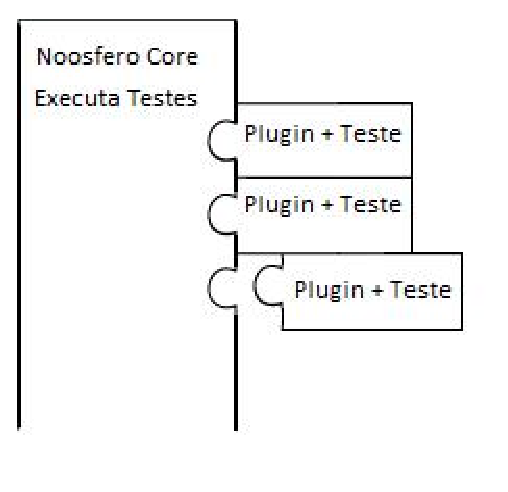
\includegraphics[keepaspectratio=true,scale=0.6]{figuras/plugins.eps}
	\caption{Arquitetura de plugins do Noosfero}
\end{figure}

Essa arquitetura é muito benéfica à implantação do Noosfero em diferentes
contextos, como por exemplo, um ambiente social virtual para economia
solidária ou um ambiente de colaboração virtual com foco no conhecimento
científico colaborativo. Os dois ambiente compartilham de um núcleo
comum a todas as redes sociais, mas diferem no uso de \textit{plugins}
com funcionalidades próprias às suas necessidades específicas.

A comunidade que colabora com o Noosfero presa muito pela qualidade
do código e por isso exige um certo nível de testes antes de aprovar
uma contribuição tanto no \textit{core} quanto em algum de seus
\textit{plugins}. A Figura \ref{plugins} apresenta a arquitetura
expansível do Noosfero.

